\externaldocument{tech_eclipse_text}

\subsection{Results \label{results}}
Overall, the program does a good job of recovering the input brightness values and matching the light curves fairly independent of the level of noise. One important thing to note is that the program does not recover the correct brightness values every time, but does a good job when averaged over many windows. This means that the results are better interpreted as long term trends than as exactly correct in every window. For the synthetic light curves, starspot evolution was not introduced. However, in real systems starspot evolution would exist. This means that our program can give information about overall trends in starspot evolution, but it cannot be trusted to give the exact brightness values of a region for any given time step. 

In all cases, the light curve fits look good for synthetic curves and real data alike. The fit of the light curve is good irrespective of noise level in the synthetic curve. An example light curve fit is shown in Figure~\ref{LC_Fit}.
\begin{figure}[h]
	\centering
	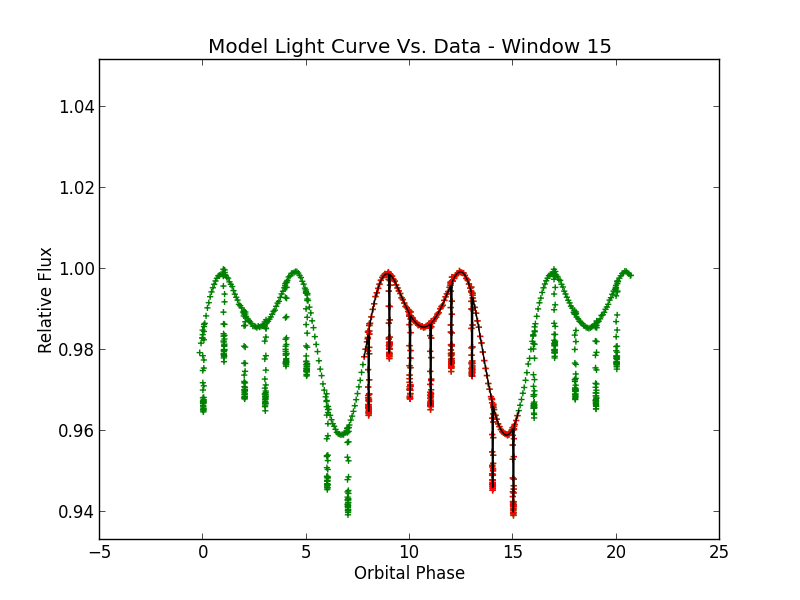
\includegraphics[width=.5\textwidth]{images/2b_2s/14_noise/model_fit_w15.png}
	\caption{Typical light curve fit produced by the Eclipse Mapping code. The green points are the overall light curve data, the red points are the data for the current window, and the black line is the model fit for that window.}
	\label{LC_Fit}
\end{figure}

To visualize the brightness values, we use Figures~\ref{stripe_plot} and~\ref{box_plot}. The value on the far right is the input value for the synthetic light curves. The y-axis in these images represents longitude along the stellar surface.

\begin{figure}[h]
	\centering
	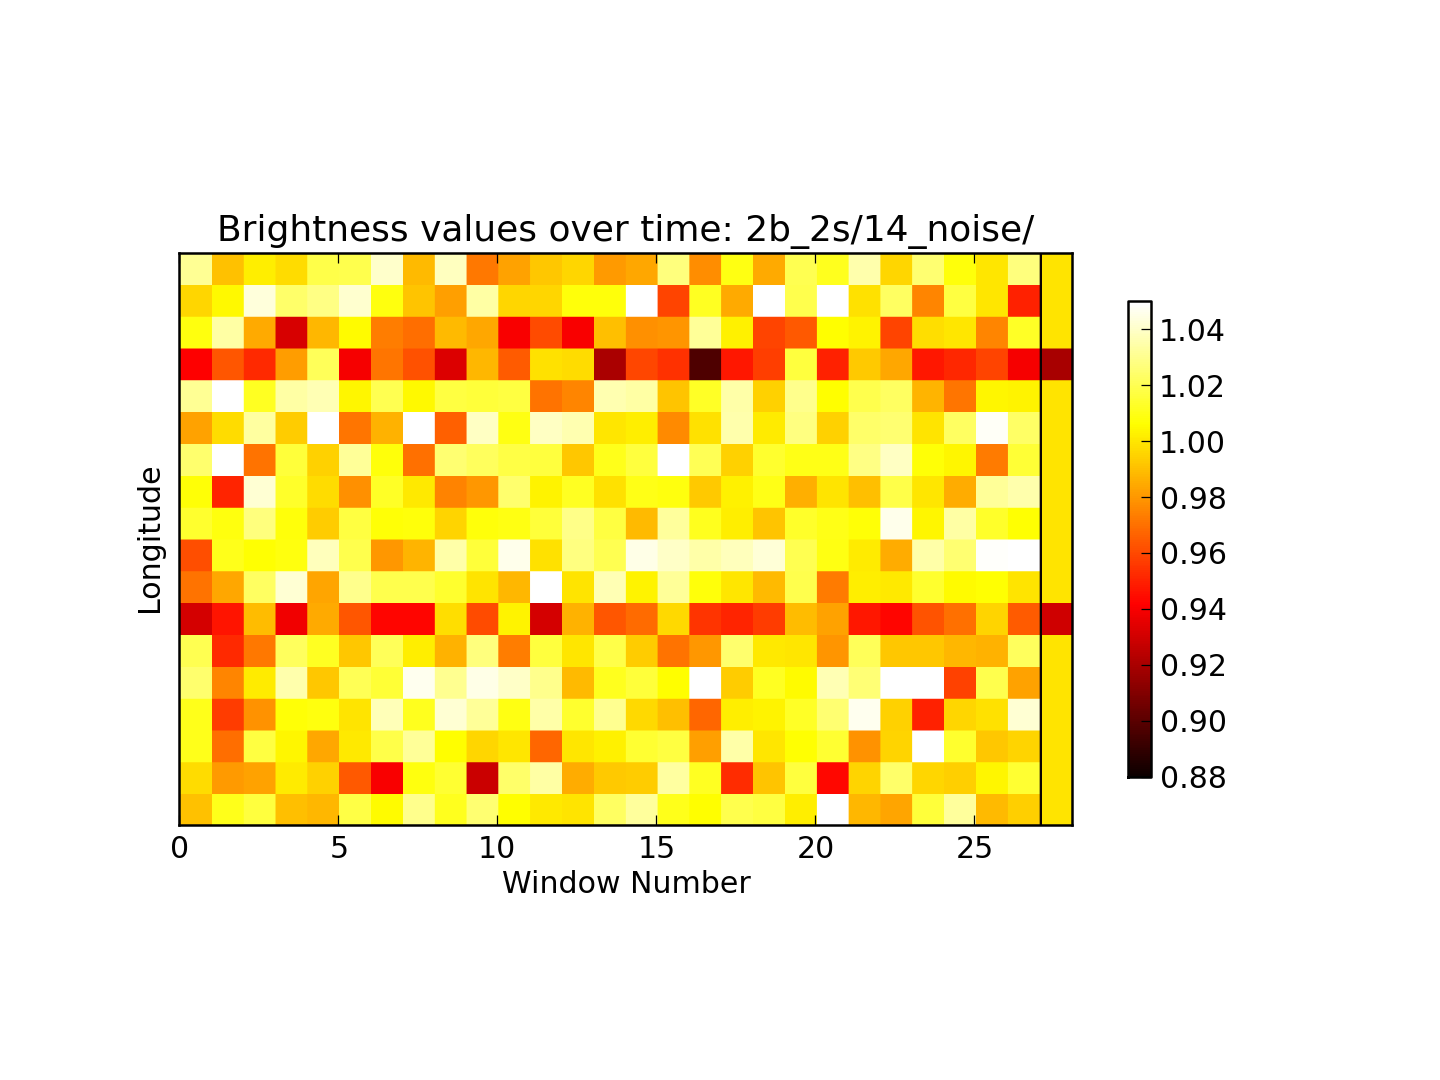
\includegraphics[width=.5\textwidth]{images/2b_2s/14_noise/box_plot.png}
	\caption{Recovered stripe brightness plot versus window number. The color bar (right) shows the relative brightness value relations to the color scale.}
	\label{box_plot}
\end{figure}
\begin{figure}[h]
	\centering
	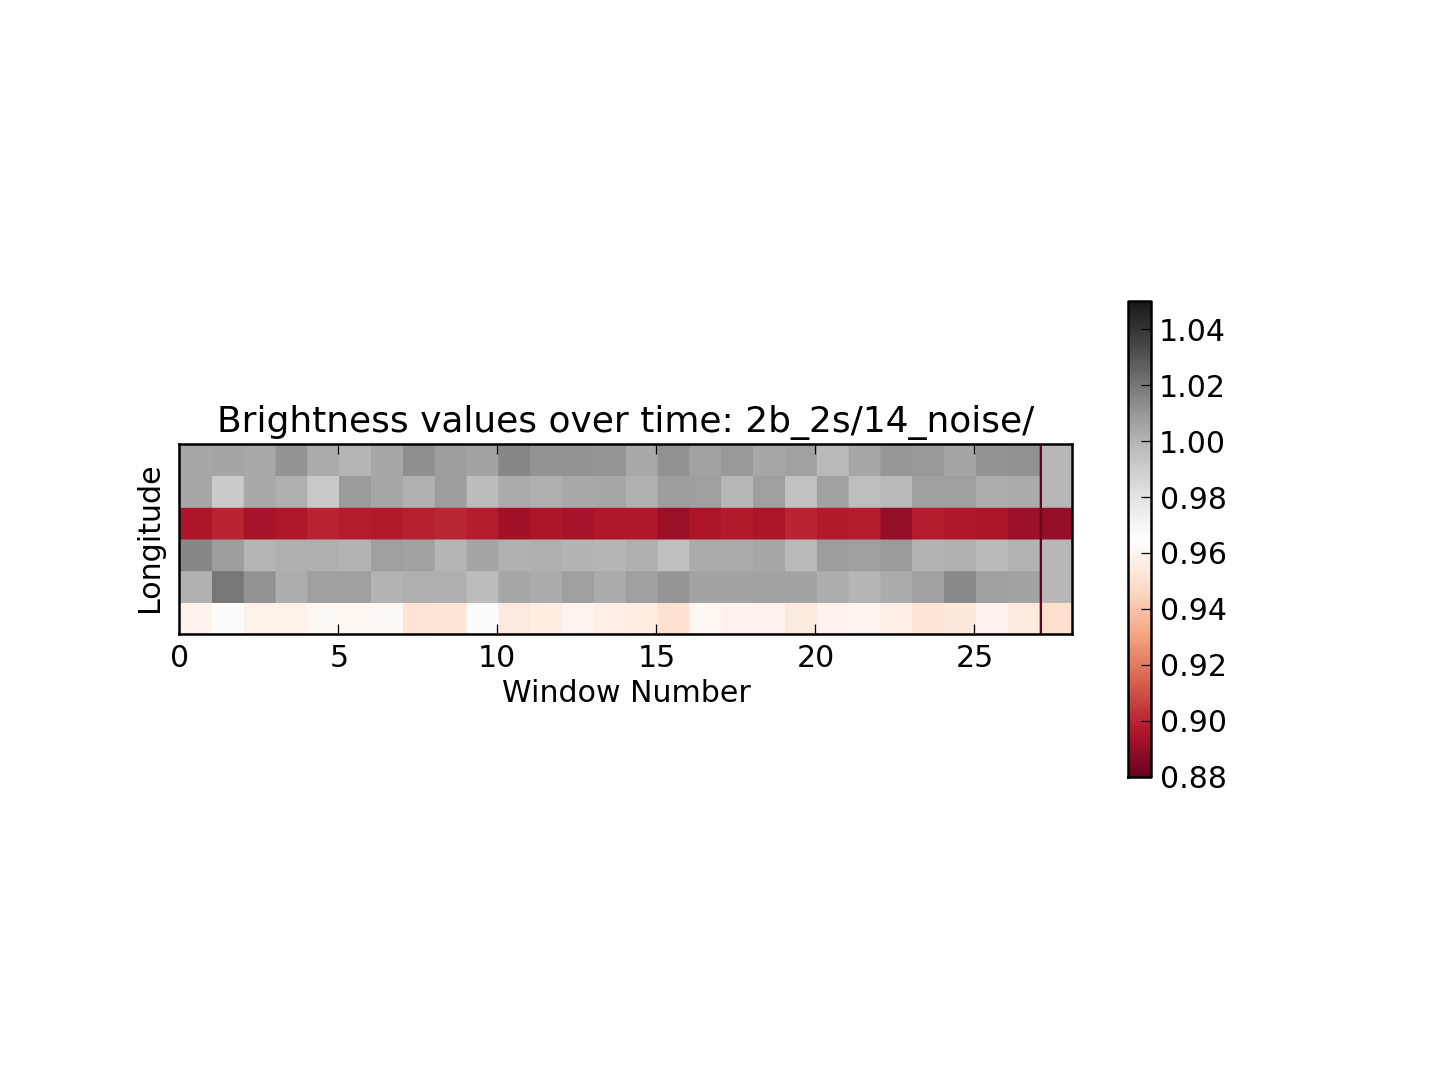
\includegraphics[width=.5\textwidth]{images/2b_2s/14_noise/stripe_plot.png}
	\caption{Recovered stripe brightness plot versus window number. The color bar (right) shows the relative brightness value relations to the color scale.}
	\label{stripe_plot}
\end{figure}

This particular set of images shows the brightness recovery for a synthetic light curve produced by darkening two stripe regions and two box regions and simulated 14th magnitude Gaussian noise. The code does a good job of recovering the brightness values for both boxes and stripes. The stripes, in general, are recovered more of the time, more precisely, and more accurately than the boxes. At any given window, one can usually believe a particular stripe measurement. The resulting stellar brightness map from this same set of recovered brightness values is shown in Figure~\ref{bright_map}.

\begin{figure}[h]
	\centering
	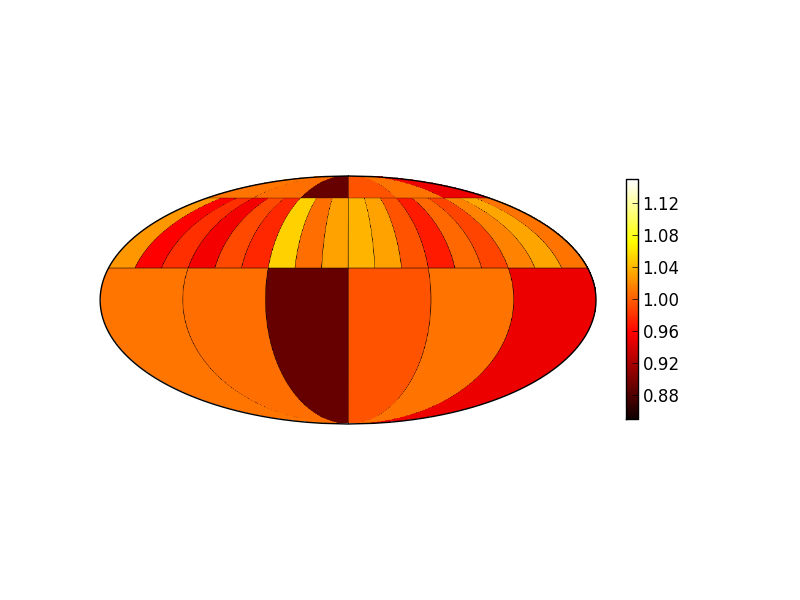
\includegraphics[width=.5\textwidth]{images/2b_2s/14_noise/brightness_map_w15.png}
	\caption{Typical stellar brightness map produced by the Eclipse Mapping code. This particular map is window 15 of the two dark stripes, two dark boxes synthetic light curve.}
	\label{bright_map}
\end{figure}